\chapter{Architecture} \label{chap:architecture}

The aim of this Chapter is to depict our system's architecture.
A high-level abstraction is presented in Figure~\ref{fig:system-architecture}, where each different component is represented together with the path data follows.
We follow a client-server organization and each functionality is designed to be modular and self-contained for the ease of deployment, evaluation, scalability and availability.

On general lines, the server-side component is executed on untrusted machines (for instance nodes on the cloud) where Intel SGX is available.
There, the \sgxspark engine is deployed and stream processes the data generated by an arbitrary number of clients using a set of medical algorithms.
Each client consists of a sensor and a gateway: the former generates samples in a continuous fashion, and the latter aggregates them and periodically sends them to the cloud-based component.
Similarly, the gateway fetches the results every fixed time intervals.
A filesystem is mounted at the server-side to interface the interaction between the clients and the processing engine.
Each client data stream is processed in parallel independently of the chosen algorithm, and results are also stored separately.

The remaining of the chapter is structured as follows: \S\ref{sec:server} details the server-side architecture, \S\ref{sec:clients} does the same with the client-side component, in \S\ref{sec:threat} we cover the considered threat model and the security assumptions we make in the design and lastly in \S\ref{sec:vulnerabilities} we present our project's known vulnerabilities.

\begin{figure}[h!]
    \centering
    \resizebox{\linewidth}{!}{
\begin{tikzpicture}
    % Colors definition: latexcolor.com
    \definecolor{ashgrey}{rgb}{0.7, 0.75, 0.71}
    \definecolor{x11gray}{rgb}{0.75, 0.75, 0.75}
    \definecolor{metal}{rgb}{0.43, 0.5, 0.5}

    
    % Main outline
    % Background
    \draw[fill=gray!10] (0, 2.75) rectangle (6.75, 6.0);

    % Client Side
    % Client boxes line
    % Client 1
    \draw[fill=gray!5] (0,1.5) rectangle (2, 2.25);
    \node at (1.6, 1.825) {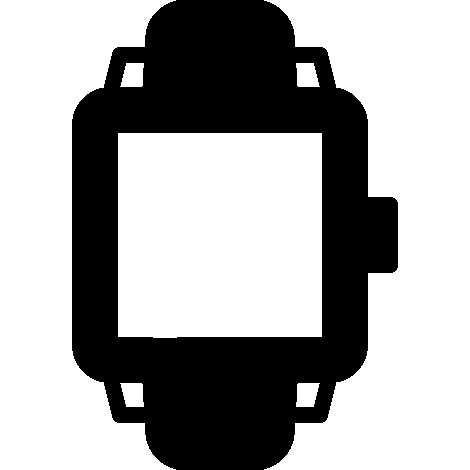
\includegraphics[width=10pt]{img/smartwatch.png}};
    \node at (1.05, 1.825) {
\includegraphics[width=10pt]{img/wifi-signal.png}};
    \node at (0.4, 1.825) {
\includegraphics[width=15pt]{img/raspberry.png}};
    % Client 2
    \draw[fill=gray!5] (2.5,1.5) rectangle (4.5, 2.25);
    \node at (2.9, 1.825) {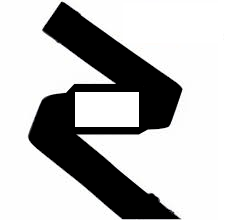
\includegraphics[width=10pt]{img/hrband.png}};
    \node at (3.5, 1.825) {
\includegraphics[width=10pt]{img/wifi-right.png}};
    \node at (4.1, 1.825) {
\includegraphics[width=15pt]{img/raspberry.png}};
    % Client 3
    \node at (5.265, 1.85) {$\cdots$};
    \draw[fill=gray!5] (5.85,1.5) rectangle (6.9, 2.25) node[pos=.5] {\tiny{Client $m$}};
    \draw[fill=gray!5] (8.875,1.5) rectangle (9.625, 2.25) node[pos=.5] {\tiny{Client}};
    % Lines to filesystem
    \draw[<->, dashed, thick] (0.4, 2.25) -- (0.4, 3.5) -- (1, 3.5);
    \draw[<->, dashed, thick] (4.1, 2.25) -- (4.1, 2.35) -- (1.35, 2.35) -- (1.35, 3);
    \draw[<->, dashed, thick] (6.3725, 2.25) -- (6.3725, 2.55) -- (1.85, 2.55) -- (1.85, 3);
    \draw[dashed, thin] (8.875, 2.25) -- (8, 2.75);
    \draw[dashed, thin] (9.625, 2.25) -- (10.5, 2.75);

    % Server Side
    % FileSystem Logo
    \draw[fill=x11gray!50] (1.0, 3) -- (1.1, 3.9) -- (1.6, 3.9) -- (1.75, 4.0) -- (2.1, 4.0) -- (2.0, 3);
    %\draw[fill=x11gray] (1.0, 3) -- (1.0, 3.8) -- (1.6, 3.8) -- (1.75, 3.6) -- (2.0, 3.6) -- (2.0, 3) -- (1.0, 3);
    \node[align=center] at (1.4, 5.1) {\text{\tiny{\textbf{FileSystem}}} \\[-8pt] \text{\tiny{\textbf{Interface}}}};
    % SGX Spark
    % Main Outline
    \draw[fill=white] (2.75, 3) rectangle (6.25, 5.5);
    \node at (4.4, 5.7) {\text{\textbf{\tiny{SGX-Spark Engine}}}};
    % SHM
    \draw (2.95, 3.2) rectangle (6.05, 3.5) node[pos=.5] {\tiny{Host Shared Memory}};
    % Driver
    \draw[pattern=north west lines,pattern color=gray!50] (2.95, 3.7) rectangle (3.95, 4.4); 
    \node at (3.75, 4.5) {\tiny{\texttt{driver-enclave.sh}}};
    \node at (2.95, 3.7) {
\includegraphics[width=8pt]{img/intel-sgx.png}};
    \draw (2.95, 4.6) rectangle (3.95, 5.3); 
    \node at (3.35, 5.4) {\tiny{\texttt{driver.sh}}};
    % Worker
    \draw[pattern=north west lines,pattern color=gray!50] (4.15, 3.7) rectangle (6.05, 4.4);
    \node at (4.9, 3.6) {\tiny{\texttt{worker-enclave.sh}}};
    \draw (4.15, 4.6) rectangle (6.05, 5.3);
    \node at (5.55, 5.4) {\tiny{\texttt{worker.sh}}};
    % Tasks Enclave
    \draw[fill=white] (4.25, 3.8) rectangle (4.65, 4.3) node[pos=.5] {\tiny{$T_1$}};
    \draw[fill=white] (4.75, 3.8) rectangle (5.15, 4.3) node[pos=.5] {\tiny{$T_2$}};
    \node at (5.35, 4.05) {\tiny{$\cdots$}};
    \draw[fill=white] (5.55, 3.8) rectangle (5.95, 4.3) node[pos=.5] {\tiny{$T_N$}};
    \node at (6, 3.7) {
\includegraphics[width=8pt]{img/intel-sgx.png}};
    % Tasks Outside Enclave
    \draw (4.25, 4.7) rectangle (4.65, 5.2) node[pos=.5] {\tiny{$T_1$}};
    \draw (4.75, 4.7) rectangle (5.15, 5.2) node[pos=.5] {\tiny{$T_2$}};
    \node at (5.35, 4.95) {\tiny{$\cdots$}};
    \draw (5.55, 4.7) rectangle (5.95, 5.2) node[pos=.5] {\tiny{$T_N$}};

    % CSEM's Toolbox
    \draw[fill=white] (0.8, 3.7) rectangle (2.1, 4.75);
    \node at (1.45, 4.55) {\textsc{\tiny{CSEM HRV}}};
    \draw[dashed] (0.8, 4.4) -- (2.1, 4.4);
    \node[align=left] at (1.42, 4.25) {\texttt{\tiny{+ Identity}}};
    \node[align=left] at (1.19, 4.05) {\texttt{\tiny{+ SDNN}}};
    \node[align=left] at (1.42, 3.85) {\texttt{\tiny{+ HRVBands}}};
    \draw[fill=x11gray] (1.0, 3) -- (1.0, 3.8) -- (1.6, 3.8) -- (1.75, 3.6) -- (2.0, 3.6) -- (2.0, 3) -- (1.0, 3);

    % Client Expansion
    % Separator
    \draw (7.3, 1.5) -- (7.3, 6);
    \draw (7.5, 1.5) -- (7.5, 6);
    % Client itself
    \draw[fill=gray!10] (8, 2.75) rectangle (10.5, 5.55);
    %\draw (9.25, 1.3725) circle (0.5);
    \draw[dashed] (8, 3.55) -- (10.5, 3.55);
    \draw[fill=white] (8.2, 2.95) rectangle (10.3, 3.35) node[pos=.5] {\tiny{\texttt{sensor}}};
    \node at (10.3, 3.00) {
\includegraphics[width=10pt]{img/docker.png}};
    \node at (8.2, 3.00) {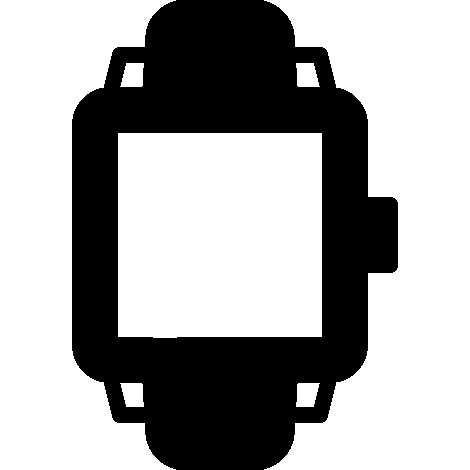
\includegraphics[width=8pt]{img/smartwatch.png}};
    \draw[fill=white] (8.2, 3.75) rectangle (10.3, 4.15) node[pos=.5] {\tiny{\texttt{eclipse-mqtt}}};
    \node at (10.3, 3.80) {
\includegraphics[width=10pt]{img/docker.png}};
    \draw[fill=white] (8.2, 4.35) rectangle (10.3, 4.75) node[pos=.5] {\tiny{\texttt{mqtt-subscriber}}};
    \node at (10.3, 4.40) {
\includegraphics[width=10pt]{img/docker.png}};
    \draw[fill=white] (8.2, 4.95) rectangle (9.2, 5.35) node[pos=.5] {\tiny{\texttt{consumer}}};
    \node at (8.3, 5.00) {
\includegraphics[width=10pt]{img/docker.png}};
    \draw[fill=white] (9.3, 4.95) rectangle (10.3, 5.35) node[pos=.5] {\tiny{\texttt{producer}}};
    \node at (10.3, 5.00) {
\includegraphics[width=10pt]{img/docker.png}};
    \draw[->, very thick, dashed] (9.8, 5.35) -- (9.8, 6);
    \draw[<-, very thick, dashed] (8.7, 5.35) -- (8.7, 6);

\end{tikzpicture}}

    \caption[Schematic of the system's main architecture.]{(Left) Schematic of the system's main architecture. A set of clients bidirectionally stream data to a remote server. The interaction is done via a filesystem interface. On the server side, \sgxspark performs secure processing using different HRV analysis algorithms. (Right) Breakdown of a packaged client: it includes a \texttt{sensor} and gateway that wrap four different microservices (\textsc{mqtt} broker, \texttt{mqtt-subscriber}, \texttt{consumer}, \texttt{producer}) to interact with the remote end. \label{fig:system-architecture}}
\end{figure}

\section{Server-Side} \label{sec:server}

The server-side component is made by three different modules: a filesystem interface, the \sgxspark engine, and a set of algorithms to analyze HRV. 
The filesystem interface acts as a landing point for the batches of data generated by each client and also stores the algorithm results.
This way, the gateway can fetch with the desired frequency the processed information.
Currently, the filesystem is mounted and unmounted, respectively at start-up time and upon the shutdown of the service. 
\sgxspark monitors the directory and processes new data as it is loaded.

The streaming engine and the pool of algorithms are compiled together by the same toolchain, yet they are independent. 
A \textsc{Spark} job deployed in standalone mode executes: the master process for resource management and allocation (not included in Figure \ref{fig:system-architecture}), a driver process that orchestrates the execution, and an arbitrary number of worker processes executing tasks.
In the case of \sgxspark jobs, two Java Virtual Machines (JVMs) are deployed per driver and worker process: one inside an enclave and one outside.
The communication between \acrshort{jvm}s is kept encrypted and is done through the host OS shared memory (see Figure \ref{fig:sgx-spark-scheme}).
A process outside the enclave never sees data in clear since sensitive operations are \emph{always} executed in secured environments.
Note that, for each newly deployed worker, a new pair of \acrshort{jvm}s and a new enclave are also deployed.

\sgxspark requires that algorithms are compiled together with the engine so that code can be loaded inside enclaves.
However, the specific algorithm that we will execute is currently set at start-up time.
It is important to note that each client has its own dedicated data stream assigned, hence being able to choose different algorithms.
These will be executed concurrently, each yielding separated results. 

\section{Clients} \label{sec:clients}

The client is a combination of: a sensor that constantly generates data, and a gateway that interacts with the remote end (see the right hand side (RHS) of Figure \ref{fig:system-architecture}). 
For evaluation purposes, the sensor component is replaced by a synthetic data generator that simulates samples.
As introduced in \S\ref{sec:background:med} and depicted in Figure \ref{fig:ecg-hrv}, the samples produced correspond to RR intervals and their timestamps.
The data generator (or fake sensor) streams samples to the gateway which is composed of: a broker and subscriber that receive the samples, a producer that aggregates them, generates files of a fixed size, and streams them to the filesystem interface, and lastly a consumer that fetches the processed data from the remote endpoint. 
To get a grasp on the volume of data a single client generates, each sample is a couple of bytes and a healthy individual generates between 50 and 180 samples per minute.
As a consequence, an average client generates around 230---690 Bytes of data per minute.
This is indeed a low throughput but, as shown in Chapter \ref{chap:implementation}, the system can withhold way higher loads.

\section{Threat Model} \label{sec:threat}

In this Section we cover our threat model and the main security assumptions we make.
This is, what kind of attacker our system is protected from.
Vulnerabilities out of the scope of this project, together with known issues are covered in \S\ref{sec:vulnerabilities}.
Firstly, we assume that the communication between the gateway and the filesystem is kept protected (\emph{e.g.}, encrypted) using secure transfer protocols (\textit{e.g. Secure File Transport Protocol (SFTP)}, more in Chapter~\ref{chap:implementation}).
Secondly, we trust the whole client package.
Protecting it is out of the scope of this work, but suggestions are given in Chapter \ref{chap:future-work}.
Given these assumptions, our threat model is the same as typical systems that rely on \textsc{SGX}. 
Specifically, we assume an attacker with access to system's privileged software such as the OS, VMM or BIOS.
Our security perimeter only includes the internals of the CPU package and the \textit{on-die} memory.
Most notably, the system's main memory (DRAM) is left \emph{outside} our security perimeter.
As a consequence, the traffic between enclave applications and main memory is kept encrypted and is handled by the MEE~\cite{Gueron16}.
The trusted computing base is Intel's microcode and the code loaded at the enclave, which can be measured and integrity checked. 
It is worth noting that, any bug or security leak included in the application code loaded in the enclave might compromise our security model.

\section{Known Vulnerabilities} \label{sec:vulnerabilities}

%Given the threat model and our particular assumptions described in \S\ref{sec:threat}, this project, \sgxspark and \sgx share an attacker model.
%As a consequence, they are all vulnerable to the same kind of attacks.
The threat model described in \S\ref{sec:threat} is the same of \sgx.
As a consequence, and given our security assumptions, it is sufficient to look into the known vulnerabilities of the latter.
Providing protection from attacks outside of \sgx's threat model is out of the scope of this project.
Intel's MEE is not designed to be an oblivious RAM, therefore an adversary could perform traffic analysis attacks~\cite{Gueron16} against our system.
This is, even if communication between the CPU and the DRAM is kept encrypted, a smart attacker could infer information from patterns in the message exchanges.
However, current work enables oblivious computations on enclaves~\cite{Zheng2017}. 
In March 2017, Schwarz \textit{et. al.}~\cite{Schwarz2017} unveiled a side-channel timing attack capable of extracting a full RSA key from an enclave in under 5 minutes.  
Not long after, various countermeasures were made available~\cite{Brasser2017,Gruss2017}.
Speculative execution attacks (\textit{Spectre}-like~\cite{Kocher2018}) have also proven to be successful against enclaves~\cite{sgx-spectre}. 
Lastly, \textit{Foreshadow}~\cite{VanBulck2018} is another speculative execution attack stronger than its predecessors and specifically targeted against Intel \sgx.
